\documentclass{article}
\usepackage{ctex}
\usepackage{graphicx}
\title{Assignment Report}
\author{牟金明 19171213839}
\date{2019.10.05}

\begin{document}
	\maketitle
	\section{Assignment1}
	Requirment:Reproduce plots 2 a,c and 3 a,c.
	
	Results are shown in Figure1 and Figure2.
	\begin{figure}[ht]
		\centering
		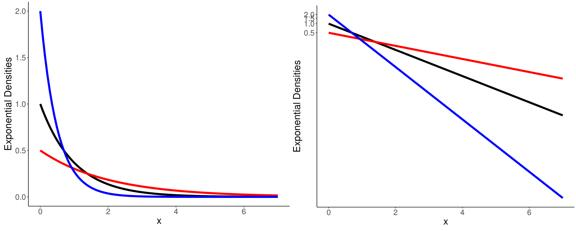
\includegraphics[scale=1]{exp.jpg}
		\caption{Exponential Densities and Semilog}
		\label{fig1}
	\end{figure}
	\begin{figure}[ht]
		\centering
		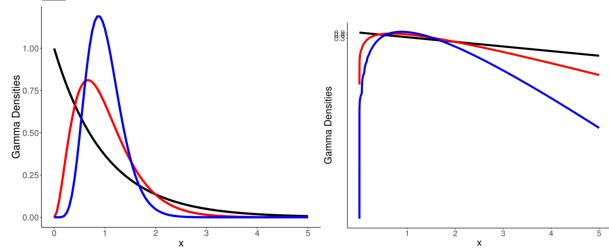
\includegraphics[scale=1]{gamma.jpg}
		\caption{Gamma Densities and Semilog}
		\label{fig2}
	\end{figure}
	
	\maketitle
	\section{Assignment2}
	Requirment:Improve these plots further using ggplot2 and the melt function;take due care of legends.
	
	Results are shown in Figure3 and Figure4.
	\begin{figure}[ht]
		\centering
		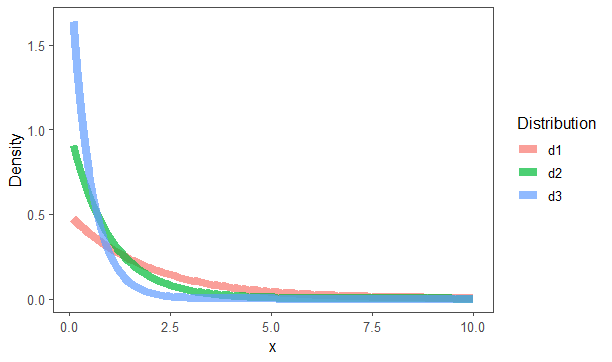
\includegraphics[scale=1]{exp2.png}
		\caption{Exponential Densities}
		\label{fig3}
	\end{figure}
	\begin{figure}[ht]
		\centering
		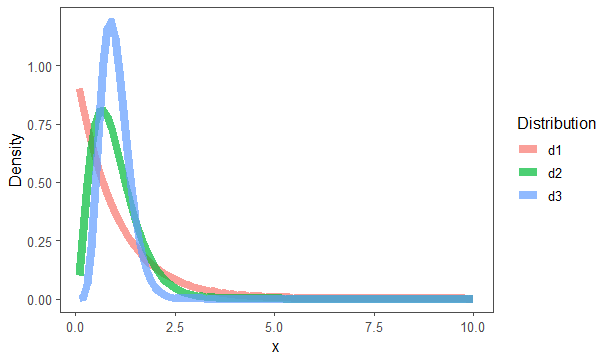
\includegraphics[scale=1]{gamma2.png}
		\caption{Gamma Densities}
		\label{fig4}
	\end{figure}

	\maketitle
	\section{Assignment3}
	Requirment:Plot densities of the K and G0 distributions.
	
	Results are shown in Figure5 and Figure6.
	\begin{figure}[ht]
		\centering
		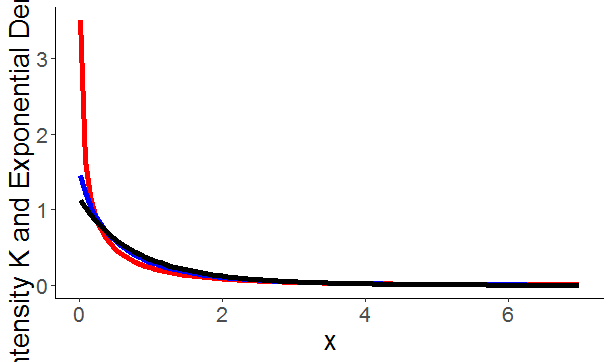
\includegraphics[scale=0.8]{K.png}
		\caption{K distribution}
		\label{fig5}
	\end{figure}
	\begin{figure}[ht]
		\centering
		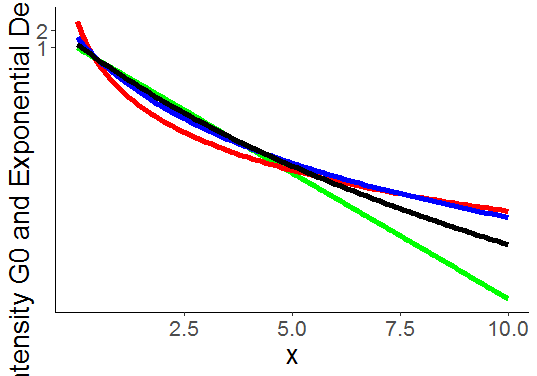
\includegraphics[scale=0.7]{G0.png}
		\caption{G0 distribution}
		\label{fig6}
	\end{figure}

	\maketitle
	\section{Assignment4}
	Requirment:Select a sample from either urban or forest from the image shown in Fig. 3.4, and repeat the analysis presented in class. 
	
	I chose urban area to analyze and the size of the example is 100*100.The example is shown in Figure7.
	
	\hspace{1cm}HH
	                 
	Min.   :       5  
	
	1st Qu.:   49397  
	
	Median :  139494  
	
	Mean   :  486161  
	
	3rd Qu.:  382280  
	
	Max.   :34400251  
	
	\begin{figure}[ht]
		\centering
		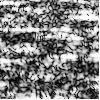
\includegraphics[scale=1]{example.png}
		\caption{Urban area}
		\label{fig7}
	\end{figure}
	
	The histogram shows in Figure8.
	
	And the result of  LogLikelihood is -3.866783e+00  1.080319e+06
	
	\begin{figure}[ht]
		\centering
		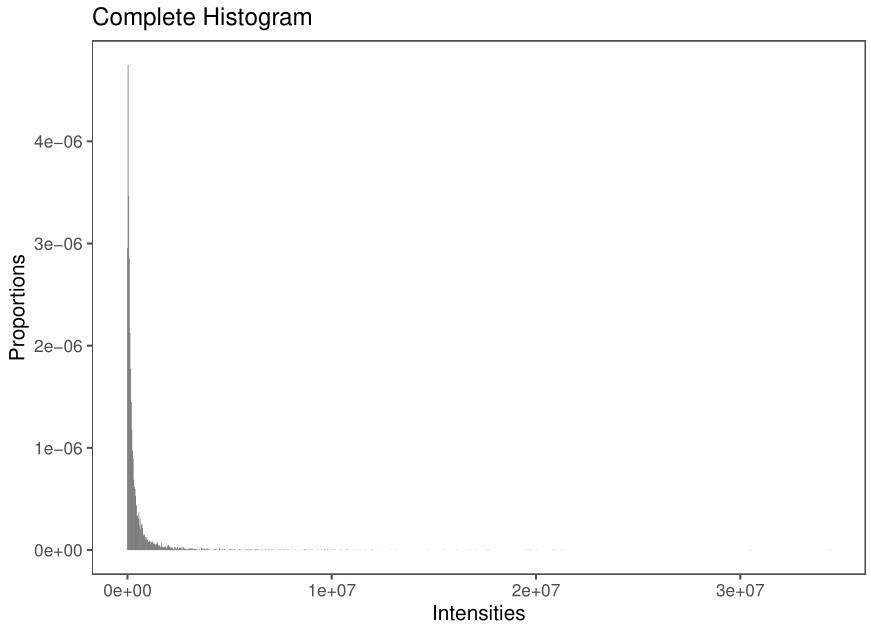
\includegraphics[scale=0.6]{histogram.jpg}
		\caption{Histogram}
		\label{fig8}
	\end{figure}

\end{document}

